\documentclass[18pt]{article}
\usepackage[utf8]{inputenc}
\usepackage[T1]{fontenc}
\usepackage{ragged2e}
\usepackage{caladea}
\usepackage{graphicx}
\usepackage{longtable}
\usepackage{wrapfig}
\usepackage{rotating}
\usepackage{epigraph}
\usepackage[normalem]{ulem}
\usepackage{hyperref}
\usepackage{amsmath}
\usepackage{amssymb}
\usepackage{capt-of}
\usepackage{hyperref}
\usepackage{fancyhdr}

\title{
 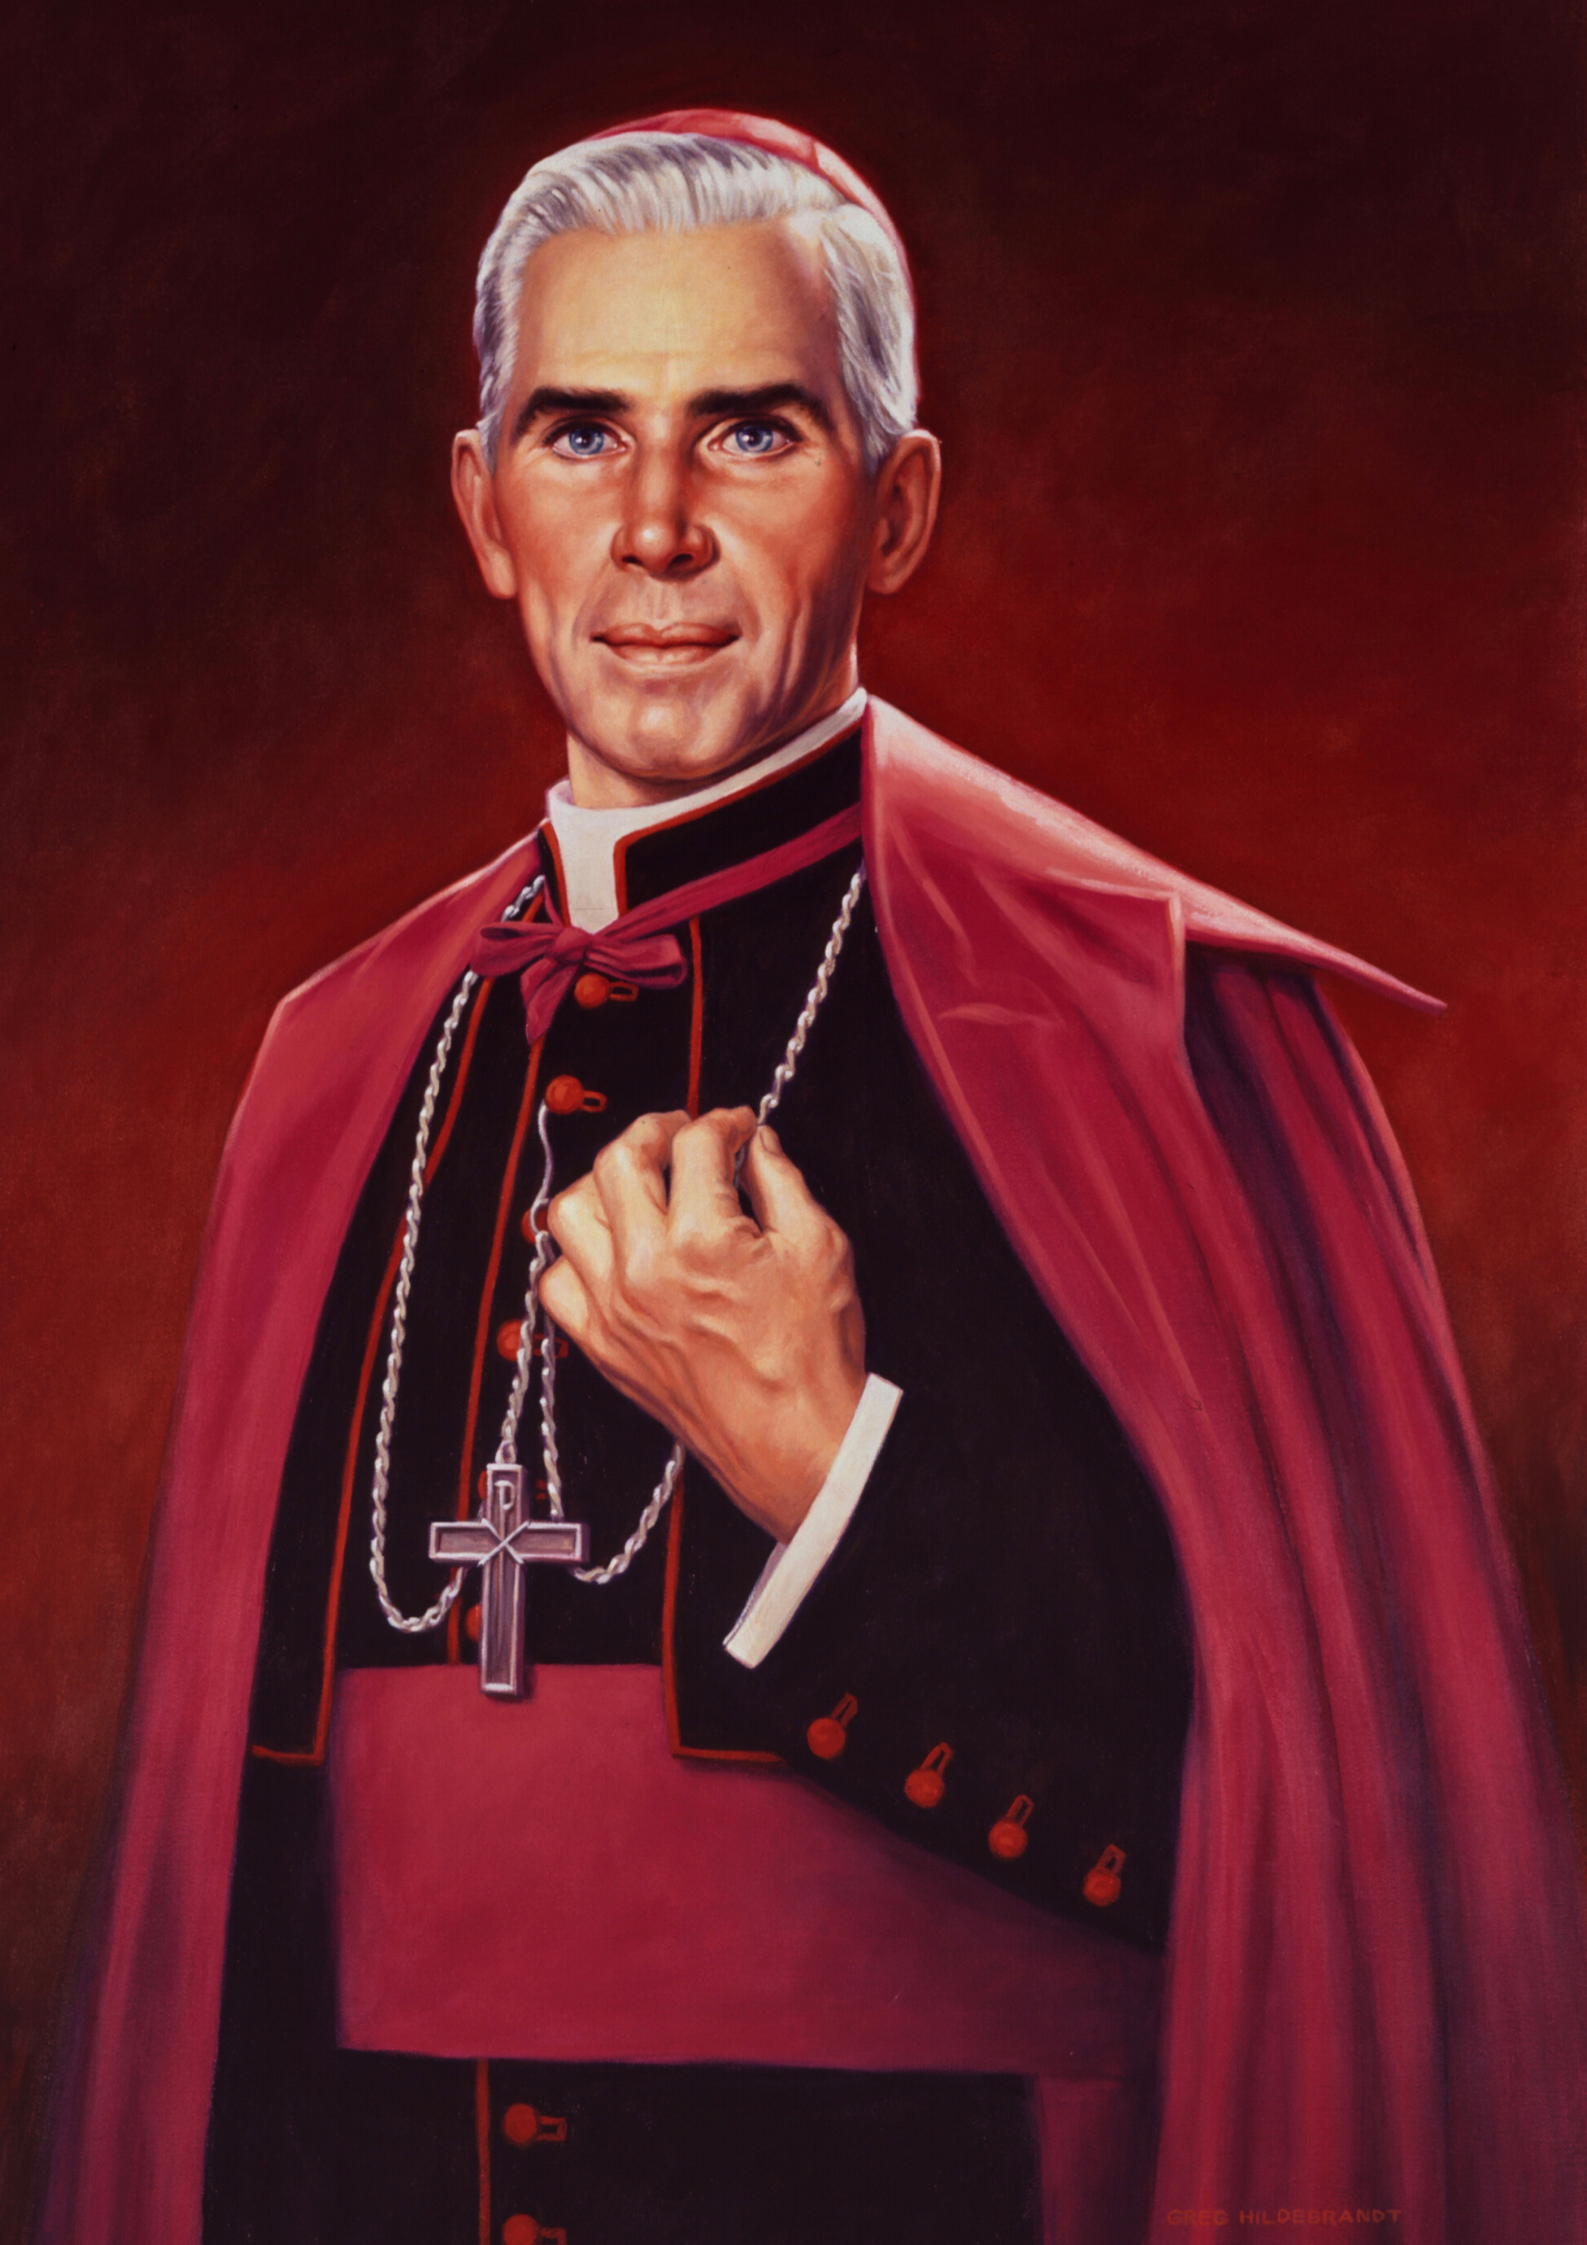
\includegraphics[scale=.55, trim={10cm, 0, 10cm, 0}]{./assets/imagem.jpg}
  \par
   NOVENA DA SÚPLICA ÀS 7 DORES E ALEGRIAS DE SÃO JOSÉ}
  \date{Início da Novena : 10/03 - Data Litúrgica: 19/03} 
  \author{Garamog, Nina Freitas}


% Comando para fazer "Sumário" não aparecer no Sumário.
\renewcommand{\contentsname}{Sumário}

\begin{document}

\thispagestyle{empty} %zera a primeira página

\maketitle

\begin{center}
 Visite-nos no Telegram: \url{https://t.me/CotidieNovena}
\end{center}

\pagestyle{fancy}
\fancyhf{} % clear existing header/footer entries
\fancyfoot[LO, CE]{
\includegraphics[scale=0.2]{./assets/cross.png} São José, rogai por nós! }
% Place Page X of Y on the right-hand
% side of the footer
\fancyfoot[R]{\thepage}

\centering
\vfill

%%%%%%%%%%%%%%%%%%%%%%%%%%%%%%%%%%%%% Orações %%%%%%%%%%%%%%%%%%%%%%%%%%%%%%%%%%%%%%%%%%%
\begin{justify}

\begin{center}
 \section*{Orações}\label{sec:Orações} % (fold)
\textit{Em nome do Pai, e do Filho, e do Espírito Santo. Amém.}
\end{center}

\subsection*{Oração Inicial}
Senhor, oferecemos esses 7 Pai Nossos e estas 7 Ave Marias em honra das 7 alegrias e das 7 dores de São José, pedindo e agradecendo seu amparo em nossas vidas, e pedindo particularmente por esta intenção: (dizer o pedido).


\subsection*{Meditação}
Rezar \textbf{1 Pai Nosso, 1 Ave-Maria e 1 Glória Ao Pai} para cada par de dor e alegria.

\vfill
\href{https://precantur.blogspot.com/2016/03/suplica-a-sao-Jose.html}{Créditos: Thesaurus Precum}

\vfill
\begin{center}
\section*{São José, Rogai por nós!}
\end{center}


\vfill


\end{justify}

\end{document}
